\documentclass[11pt, a4paper]{article}
\usepackage[spanish]{babel}
\usepackage[T1]{fontenc}
\usepackage[UTF8]{inputenc}
\usepackage{graphicx, amsmath, booktabs, latexsym, mathrsfs, amssymb, amsthm, units, siunitx, textcomp,subcaption,wrapfig,enumerate}
\usepackage{anysize}
\marginsize{1.5cm}{2cm}{1.5cm}{2cm}

\begin{document}
\title{Uso de motores y servos en Robótica \\ {\Large Robótica y Mecatrónica}}
\author{Arcadi Garcia, Melodía Moya} \date{}
\maketitle

\section{Cuestiones a realizar}
		\begin{enumerate}[(a)]
			\item \textbf{Observar cómo afecta la luz externa en la detección.}
			
			Si hay mucha luz, ésta puede atravesar el papel y provocar un aumento en las lecturas de los sensores. Como son sensores infrarrojos, dependiendo del tipo de luz, este efecto será mayor con luz solar, que tiene una mayor componente infrarroja, la cual puede dar lugar a falsos "blancos", que con luz proveniente de los fluorescentes, por ejemplo.
En cambio, si la iluminación externa es baja la única luz que le puede llegar al sensor es la reflexión de la propia luz infrarroja que él mismo emite.

Es por eso que hemos colocado los sensores en la parte baja del robot, de manera que se proteja a sí mismo de las interferencias debidas a la luz externa.

			\begin{figure}[h!]
				\centering
				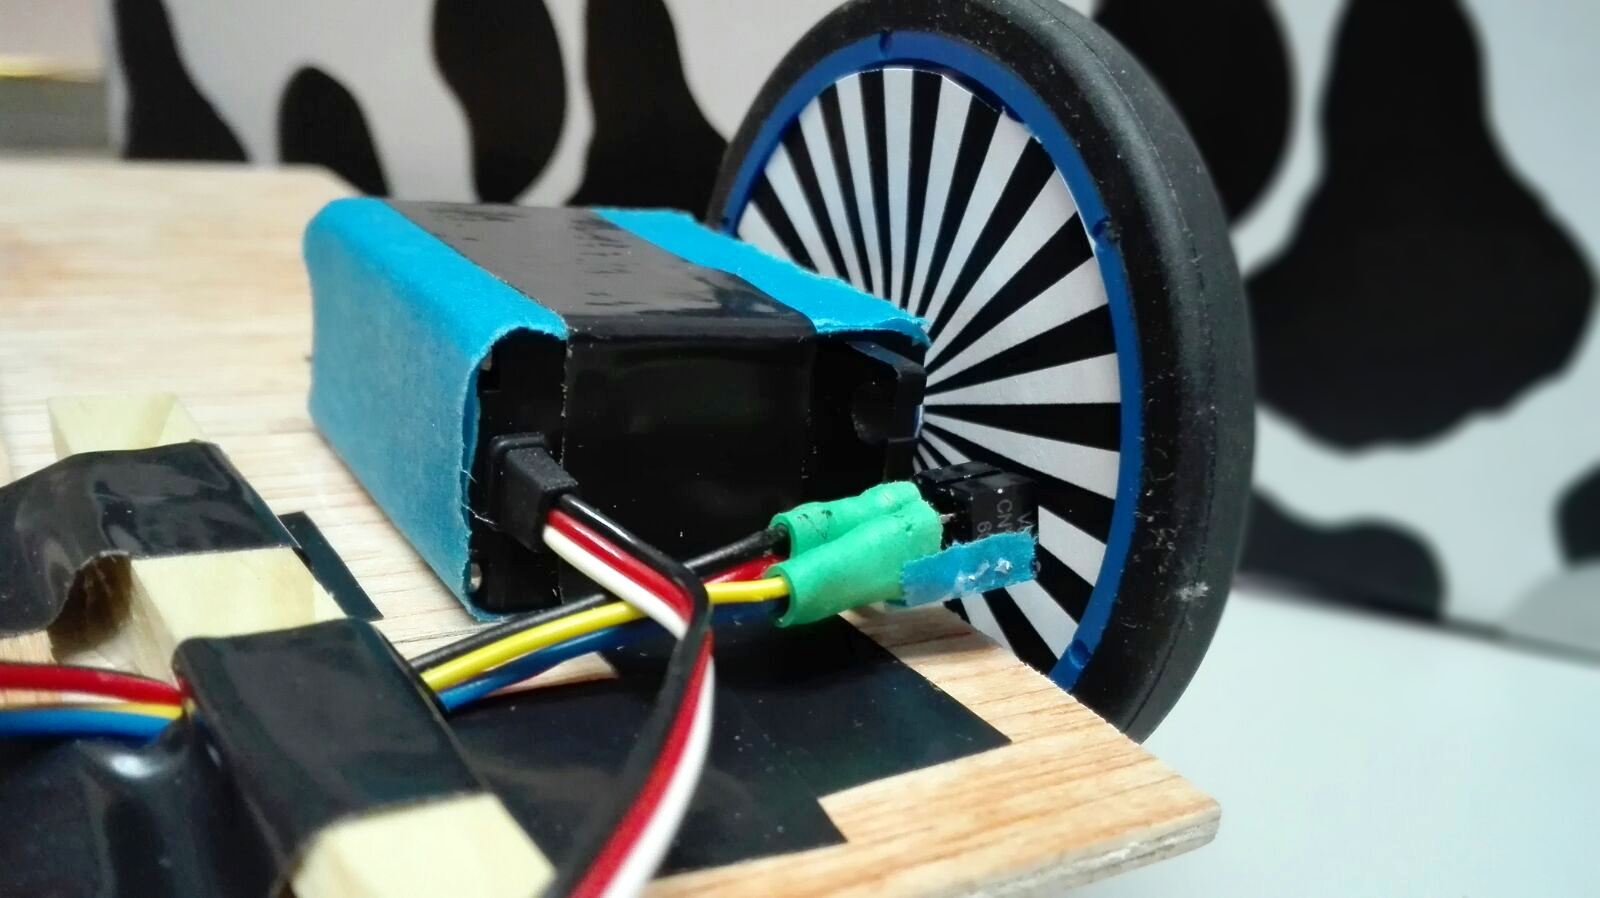
\includegraphics[width=.9\textwidth]{encoder}
				\caption*{Colocación del sensor del encoder en la parte inferior del robot, junto a los motores.}
			\end{figure}

			\item \textbf{Comprobar el rango de funcionamiento del sensor. Verifique los niveles de intensidad que obtiene y calibre hasta cuando puede medir y no confundirlo con la señal del entorno, es decir, encuentre la relación señal/ruido que pemite su uso en el encoder.}
			
			El sensor tiene que medir dos facetas del encoder: cuando se halla en un blanco o en un negro. Midiendo con un multímetro, medimos que el blanco pulula por el rango de $2.5 - 3$ V, mientras que el negro lo hace alrededor $0.5 - 1.3 V$. Dejando el sensor mirando hacia el infinito, medimos hasta $0.3$ V.
			
			Sacando las relaciones señal-ruido, obtenemos:
			
			$$ SNR = \dfrac{blanco - negro}{fondo} = \dfrac{2.75 V - 0.35 V}{0.3 V} = 8 $$
			
			Esto nos da una relación señal-ruido bastante buena. Podemos incluso, teóricamente, funcionar por umbrales. No obstante, hay que tener en mente que la realidad con un encoder en movimiento será más difusa y más compleja de interpretar.
			
			\item \textbf{Comprobar cómo afecta el tipo de superficie de los objetos sensados en la medida.}
	
			Cuanto más rugosa sea la superficie, más luz dispersará y menor será la potencia del haz reflejado que llegará al detector. Lo mismo ocurre en el caso de superficies muy absorbentes o muy transparentes, ya que tendrán una reflectividad muy baja.
			
			\end{enumerate}
			
\section{Códigos}
	\subsection{Sensores}
	 El archivo encargado de interpretar las lecturas del ADC y mantenerse alerta por si aparecen obstáculos es \textit{sense.c}:
	 
	 \begin{verbatim}
	 	#include <wiringPi.h>
#include <stdio.h>
#include <pthread.h>

#define SPIOUT 13
#define UMBRAL 620
#define FRANJAS 48
#define LUT_SIZE 17

static unsigned char dist[LUT_SIZE] = {3, 4, 5, 6, 7, 8, 9, 10, 12, 14, 16, 18, 20, ...
... 25, 30, 35, 40};
static float volt[LUT_SIZE] = {3.0348, 2.7261, 2.3478, 2.0347, 1.7826, 1.5869, 1.4, ...
								... 1.2956, 1.0913, 0.9608, 0.8478, 0.7739, 0.6565, 0.5217, 0.4304, 0.3739, 0.313};

float dista[2];
//lee el sens-ésimo sensor del encoder (0 ó 1)
char leeSens(int sens){
    int x = analogRead(100+sens);
    if(x>UMBRAL){ //devolvemos blanco (1) o negro (0) en función de la lectura del sensor
        return 1;
    } else {
        return 0;
    }
}

//lee el sens-ésimo sensor del encoder (2 ó 3)
float leeIR(int sens){
    
	short val = analogRead(100+sens);
	float v = 3.3*((float)val)/1024.0;

	// LEEMOS EL SENSOR IR
	float d=-1;
	int i=0,pos=0;
	float vol1, vol2, d1, d2;

    //Buscamos a qué posición del vector volt estamos
    while(v<volt[i] && i<LUT_SIZE){
        pos++;
        i++;
    }
    
    if(!(pos==0 || pos>=LUT_SIZE)){
        vol1 = volt[pos-1];
        vol2 = volt[pos];
        d1 = (float)dist[pos-1];
        d2 = (float)dist[pos];

        d = d1 + (v-vol1)*(vol2-vol1)/(d2-d1);
    }
        
    return d;
}

PI_THREAD(distance){ //va midiendo distancias cada medio segundo
    while(1){
        dista[0] = leeIR(2);
        dista[1] = leeIR(3);
        delay(500);
    }
}

//inicializa el hilo
void sensoresSetup(){
    dista[0] = leeIR(2);
    dista[1] = leeIR(3);
    int x = piThreadCreate(distance);
}

	 \end{verbatim}

	\subsection{Motores}
		El archivo encargado de gestionar los motores y estabilizar el movimiento con la ayuda de los encoders es \textit{move.c}:
		
		\begin{verbatim}
			#include <stdio.h>
#include <wiringPi.h>
#include <softPwm.h>
#include "sense.h"
#include <pthread.h>
#include <stdlib.h>

/* Definimos todas las especificaciones del robot */
#define PINR 0 // Pin para la rueda derecha
#define PINL 1 // Pin para la rueda izquierda
#define PERIIZQ 0.22 //Perímetro (en m) de las ruedas.

//Qué valores pasar al PWM y demás cosis.
#define FWL 20
#define FWR 5
#define BKL 10
#define BKR 25

//Vueltas/segundo de cada rueda
#define FWLV 0.860585
#define FWRV 0.8365
#define BKLV 0.9208
#define BKRV 0.8421

//Vueltas/segundo del giro global
#define SPIN 0.326 //rev/s
//Velocidad (grosso modo) de avance del robot.
#define SPEED 0.174 //m/s
//s/vuelta pivotando
#define PIVL 7.52
#define PIVR 7.2

//Variables globales para los hilos
int fri=0, frd=0; //franjas recorridas
char sti, std; //franja actual (0 = negro, 1 = blanco)
char sensen=0, correcting=0; //permite contar

void startCounting(){
    sensen = 1;
    fri = 0;
    frd = 0;
    sti = leeSens(0);
    std = leeSens(1);
}

//Para.
void stop(){
    softPwmWrite(PINL,0);
    softPwmWrite(PINR,0);
    sensen = 0;
}

/* A continuación se escribe la función principal */
//Va hacia delante (1) o hacia atrás 0.
void gofw(int dir){
    startCounting();
    
    if(dir == 1){
        softPwmWrite(PINL,FWL);
        softPwmWrite(PINR,FWR);
    } else {
        softPwmWrite(PINL,BKL);
        softPwmWrite(PINR,BKR);
    }
}

//Va hacia delante cm cm.
void advance(int cm){
    startCounting();
    
    if(cm > 0){
        softPwmWrite(PINL,FWL);
        softPwmWrite(PINR,FWR);
    } else {
        softPwmWrite(PINL,BKL);
        softPwmWrite(PINR,BKR);
        cm = -cm;
    }
    
    delay(cm*10/SPEED);
    stop();
}

//Gira 90º en una dirección (0 IZQ ó 1 DCH)
void turn(int tow){
    int mchl, mchr;
    startCounting();
    //En función de la dirección, asignamos una marcha a cada motor.
    switch(tow){
        case 0:
            mchl = BKL;
            mchr = FWR;
            break;
        case 1:
            mchl = FWL;
            mchr = BKR;
            break;
        default:
            mchl = 0;
            mchr = 0;
    }
    
    softPwmWrite(PINL,mchl);
    softPwmWrite(PINR,mchr);
    delay(250/SPIN);
    stop();
    
}

//hilo para poder mantener el movimiento bien
PI_THREAD(stable){
    int leci, lecd;
    while(1){
        if(sensen){
            leci = leeSens(0);
            lecd = leeSens(1);
            
            //comprueba si nos hemos cambiado de franja
            if(leci != sti){
                sti = leci;
                fri++;
            }
            if(lecd != std){
                std = lecd;
                frd++;
            }
            
            //cada media vuelta, comprueba si hay discrepancias entre los motores
            // si las hay, apaga uno de los motores
            if((fri%FRANJAS/2 == 0) || (frd%FRANJAS/2==0)){ //cada media vuelta, comprueba
                if(abs(fri-frd)>FRANJAS/4 && !correcting){
                    correcting = 1;
                    //Paramos uno de los motores.
                    if(fri > frd){
                        softPwmWrite(PINL,0);
                    } else {
                        softPwmWrite(PINR,0);
                    }
                }
            }
            
            //cuando las discrepancias desaparecen, todo vuelve a la normalidad
            if(correcting && frd == fri){
                softPwmWrite(PINL,FWL);
                softPwmWrite(PINR,FWR);
                correcting = 0;
            }
        }
        delay(10);
    }
}

//inicializa el hilo
void motoresSetup(){
    sti = leeSens(0);
    std = leeSens(1);
    int x = piThreadCreate(stable);
}
		\end{verbatim}
		
	\subsection{main}
	
	Finalmente, el programa que hace lo que se nos pide (avanzar hasta encontrar un obstáculo, acercarse hasta los 20cm del mismo, girar 90º a la izquierda, avanzar 40 cm, girar 90º a la derecha, avanzar 50cm y parar) es:
	
	\begin{verbatim}
		#include <stdio.h>
#include <wiringPi.h>
#include <softPwm.h>
#include "move.h"
#include <mcp3004.h>
#include "sense.h"

#define INIVAL 0 // Valor inicial del PWM
#define RANGO 100 // Rango del PWM
extern float dista[2];

int main(){
    char who; //0 sensor izq triggered y 1 sensor dcho triggered
	wiringPiSetup(); /* Inicializamos WiringPi */
	mcp3004Setup(100,0); //Inicializamos las cosillas del ADC
    motoresSetup();
    sensoresSetup();
    
	/* Ya procedemos a crear los PWM */
	softPwmCreate(PINR, INIVAL, RANGO);
	softPwmCreate(PINL, INIVAL, RANGO);
	int izq=0, dch=0; /* Marchas PWM */
	stop();
    
	printf("Pulsa ENTER para empezar.\n");
	getchar();
    
	gofw(1);
	while(dista[0] == -1 && dista[1] == -1){}
	stop(); //para al detectar algo
    delay(10);
    if(dista[0] == -1 && dista[1] != -1){
        who = 1;
    } else if(dista[0] != -1 && dista[1] == -1){
        who = 0;
    }
    gofw(1);
    while(dista[who] > 20){}
	delay(100);
	turn(0);
    delay(100);
    advance(40);
    delay(100);
    turn(1);
    delay(100);
    advance(50);
    
	return 0;
}
	\end{verbatim}
\end{document}